\documentclass[twocolumn]{article}

\usepackage{enumerate}
\usepackage{graphicx}
\usepackage[colorlinks=true,linkcolor=blue]{hyperref}
\usepackage[table,xcdraw]{xcolor}
\usepackage[english,spanish]{babel} 
\usepackage{helvet}

\renewcommand{\familydefault}{\sfdefault}

\newenvironment{poliabstract}[1]
   {\renewcommand{\abstractname}{#1}\begin{abstract}}
   {\end{abstract}}

\begin{document}

\title{Comparativa de Frameworks de Pruebas de APIs}
\author{Herrera Amezquita,
Derian  \\Paredes Catacora, Randi \\Mejia Rodriguez, Julio\\Marco Garcia\\Alisson Chino}


\date{04 de Diciembre de 2020}

\maketitle

\selectlanguage{spanish}
\begin{poliabstract}{Resumen} 
  En el desarrollo del articulo de investigacion expondremos sobre los frameworks de pruebas de apis asi como tambien se hablara sobre lo que es una api y como funciona tambien compararemos dos frameworks de pruebas de apis.
  
\end{poliabstract}

\selectlanguage{english}
\begin{poliabstract}{Abstract} 
  In the development of the research article we will expose about the API testing frameworks as well as what an API is and how it works we will also compare two API testing frameworks.
\end{poliabstract}

\section{Introducción}
Para producir software con un nivel  de calidad  insuficiente puede ser un pésimo negocio. Según Stadish Group en su informe de 2015 ( Chaos Report)[1], el 52% de los proyectos de desarrollo de software no alcanza los objetivos deseados y el 19% de ellos se consideran fracaso.
Solo el 29\% llegan a el exito, No solo es suficiente con que una aplicación funcione completamente , acorde a su propósito , sino que también debe satisfacer otros aspectos en términos de seguridad , rendimiento, accesibilidad ,etc. Por eso el objetivo de cualquier organización que se dedique a la industria del software debe producir software de calidad .
La calidad debe ser una  exigencia obligada y cada vez son mas las empresas que consideran el aseguramiento de la calidad.
Una de las partes importantes que componen las tareas propias de un sistema de aseguramiento de la calidad que son las pruebas de software.
Existen pruebas unitarias , de integracion, funcionales, de rendimiento, etc. 
En la actualidad existen herramientas que permiten generar y ejecutar scripts, pequeños programas que permiten interactuar con una aplicacion dada , simulando las acciones que podria realizar un usuario real
, estas herramientas ayidan a incrementar la productividad como frameworks de pruebas para apis.
\section{Desarrollo}
\subsection{¿Que es un API?}
API (Application Programming Interface) Es una interfaz informatica con la cual se puede intercambiar y comunicar datos entre dos sitemas de software separado.
API incluye varias funciones / subrutinas que puede realizar otro sistema de software. La API define las solicitudes que se pueden realizar, cómo realizar las solicitudes, los formatos de datos que se pueden utilizar, etc. entre dos sistemas de software.\\

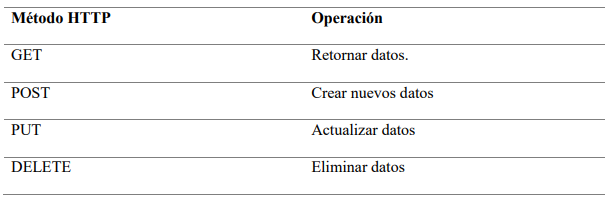
\includegraphics[width=1.02\linewidth]{img/foto1}
\subsection{API Rest}
REST (Representation State Transfer) es una arquitectura basada en red que Fielding y Row
(2000) introdujo y definió por primera vez para proporcionar interoperabilidad entre sistemas
informáticos en Internet. Una arquitectura REST se define por un conjunto de restricciones y
sus recursos se identifican mediante URI (identificadores uniformes de recursos); estos
recursos pueden representar objetos de datos como uno de varios formatos de datos como JSON
o XML.
REST utiliza el protocolo HTTP como medio de transporte para crear servicios web ligeros,
flexibles y escalables.[2]

Existen códigos diferentes, pero los siguientes son los más
comúnmente utilizados:
\\• 200 Ok: la respuesta HTTP estándar representa éxito en el retorno.
\\• 201 Created: Este código de estado debe ser devuelto cada vez que se crea la nueva
instancia. Debe ser el resultado de la solicitud POST.
\\• 400 Bad Request: indica que la solicitud del cliente no se procesó, ya que el servidor
no pudo entender lo que el cliente está pidiendo.
\\• 401 Unauthorized: indica que el cliente no puede acceder a los recursos y debe volver
a solicitar con las credenciales requeridas.
\\• 403 Forbidden: indica que la solicitud es válida y el cliente está autenticado, pero el
cliente no tiene permiso para acceder al recurso.
\\• 404 Not Found: indica que el recurso solicitado no está disponible ahora.
\\• 500 Internal Server Error: indica que la solicitud es válida, pero se produjo un error
inesperado al procesar la solicitud. (Haldar, 2017).[3]\\
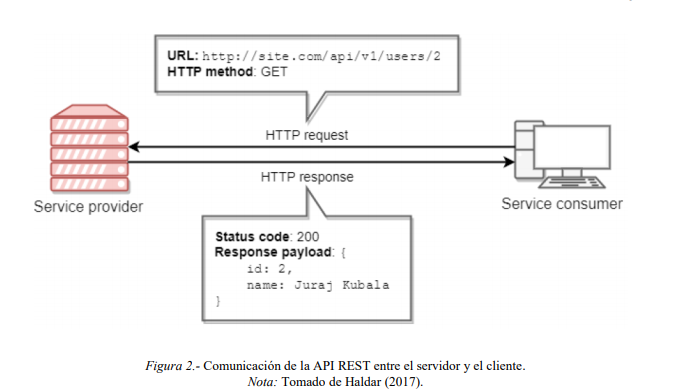
\includegraphics[width=1.02\linewidth]{img/foto2}
\newpage
\subsection{¿Qué son las pruebas de API?}
PRUEBA DE API es un tipo de prueba de software que valida las interfaces de programación de 
aplicaciones (API). El propósito de las pruebas de API es verificar la funcionalidad, confiabilidad,
 rendimiento y seguridad de las interfaces de programación. En API Testing, en lugar de utilizar 
 entradas y salidas de usuario estándar (teclado), utiliza software para enviar llamadas a la API, 
 obtener resultados y anotar la respuesta del sistema. Las pruebas de API son muy diferentes de las 
 pruebas de GUI y no se concentran en la apariencia de una aplicación. Se concentra principalmente en
  la capa de lógica empresarial de la arquitectura de software.[4]\\
  \\
  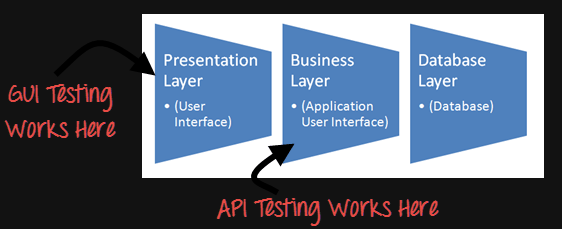
\includegraphics[width=1.02\linewidth]{img/foto3}
\subsection{Frameworks de Pruebas de APIs }

\subsubsection{Postman}
Herramienta que se utiliza, sobre todo, para el testing de API REST, aunque también admite otras funcionalidades que se salen de lo que engloba el testing de este tipo de sistemas.

Gracias a esta herramienta, además de testear, consumir y depurar API REST, podremos monitorizarlas, escribir pruebas automatizadas para ellas, documentarlas, mockearlas, simularlas, etc.
\newpage
Quizás sea una de las herramientas más utilizadas para hacer testing exploratorio de este tipo de sistemas. Puede que no sea la mejor forma de escribir pruebas automatizada, pero sin duda es una de las más favorables para equipos con poca experiencia en programación, y sobre todo para hacer testing de todo tipo en general de API REST.
[5]\\

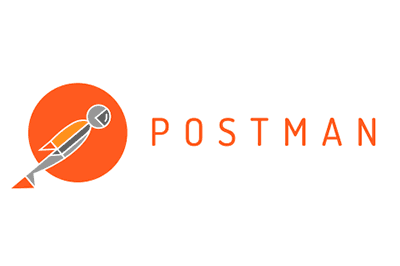
\includegraphics[width=0.8\linewidth]{img/foto4}

\textbf{Caracteristicas}
\\•Crear Peticiones, te permite crear y enviar peticiones http a servicios REST mediante un interface gráfico. Estas peticiones pueden ser guardadas y reproducidas a posteriori.

•Definir Colecciones, mediante Postman podemos agrupar las APIs en colecciones. En estas colecciones podemos definir el modelo de autentificación de las APIs para que se añada en cada petición. De igual manera podemos ejecutar un conjunto de test, así como definir variables para la colección.

•Gestionar la Documentación, genera documentación basada en las API y colecciones que hemos creado en la herramienta. Además esta documentación podemos hacerla pública.

•Entorno Colaborativo, permite compartir las API para un equipo entre varias personas. Para ello se apoya en una herramienta de colaborativa en Cloud.

•Genera código de invocación, dado un API es capaz de generar el codigo de invocacion para diferentes lenguajes de programacion: C, cURL, C\#, Go, Java, JavaScript, NodeJS, Objective\-C, PHP, Python, Ruby, Shell, Swift,etc.

•Establecer variables, con Postman podemos crear variables locales y globales que posteriormente utilicemos dentro de nuestras invocaciones o pruebas.

•Soporta Ciclo Vida API management, desde Postman podemos gestionar el ciclo de vida del API Management, desde la conceptualización del API, la definición del API, el desarrollo del API y la monitorización y mantenimiento del API.

•Crear mockups, mediante Postman podemos crear un servidor de mockups o sandbox para que se puedan testear nuestras API antes de que estas estén desarrolladas.

\newpage
\textbf{Ventajas de Postman}
\begin{itemize}
  \item Permite la colaboración entre miembros del equipo.
  \item Tiene una interfaz más intuitiva y atractiva.
  \item Posee extensión para Google Chrome,  por lo tanto no es necesario instalar la aplicación de escritorio.
  \item Como ya mencionamos en la descripción, tiene una opción muy interesante, que son las colecciones, que funciona básicamente como una base de datos de peticiones.
  \item Es extensible y se puede integrar con otras herramientas, por ejemplo ejecutando las suites de prueba desde un motor  de CI/CD.
  \item Permite agregar scripts en lenguaje Javascript para agregar validaciones, configurar y/o automatizar pruebas (esto se realiza directamente en la petición).[6]
\end{itemize}

\subsubsection{SoapUI }
SoapUI es una herramienta desarrollada en Java, utilizada para pruebas de aplicaciones con arquitectura SOA o REST. Soporta múltiples protocolos como SOAP, REST, HTTP, JMS y JDBC. La herramienta cuenta con una versión de código abierto y otra versión paga desarrollada por la compañía SmartBear.
La herramienta SoapUI se creó inicialmente para probar los servicios SOAP. Luego, se extendió a los servicios web RESTful. \\

\includegraphics[width=1.02\linewidth]{img/foto5}
\\Para un usuario nuevo puede requerir una mediana curva de aprendizaje ya que la misma en ocasiones no resulta tan intuitiva.
[7]



\newpage
\textbf{Funcionalidades}
\begin{itemize}
\item Las principales funcionalidades que aporta la herramienta soapUI son:

\item Inspecciona Web Services WSDL y REST (tanto WADL como WADLess) y los visualiza jerárquicamente.
\item Genera automáticamente los tests y las peticiones SOAP de las operaciones definidas en el descriptor WSDL o WADL.
\item Permite verificar la conformidad de un WSDL según los estándares WS-I*.
\item Opcionalmente, puede utilizarse el scripting de Groovy para que el comportamiento de los tests sea dinámico.
\item Soporta varios métodos de autentificación: Basic, Digest, WS-Security y NTLM Web Service.
\item Soporta diferentes tecnologías de ficheros adjuntos: MTOM, SOAP con Attachments, ficheros Inline para WSDL y MIME Attachments para REST.
\item Verificación del contenido de mensajes con Xpath y Xquery.
\item Versatilidad en la configuración del test de carga, pudiendo indicar el límite (en tiempo o peticiones), el número de threads de ataque, el método HTTP de la petición (POST, GET ...).
\item Permite exponer Web Services de simulación (o mocking) con el contenido de respuesta personalizable.
\end{itemize}
\newpage
\textbf{Ventajas}
\begin{itemize}
\item Es una aplicación muy completa, con muchas funcionalidades, con lo cual puede llegar a ser un poco complicada de utilizar para la función que queramos en cada momento.
\item Tiene una mejor integración que Postman para trabajar con el protocolo SOAP (ya que inicialmente estaba pensada para eso).
\item Es un proyecto más maduro y tiene más tiempo en el mercado.
\item Es una aplicación más orientada a testing y no simplemente a consumir una API, documentarla y publicarla. Permite estructurar las pruebas en test suites, test cases y test steps.
\item La ejecución de pruebas se puede integrar con herramientas tales como: Maven, motores de CI/CD, etc.
\item Permite agregar scripts en lenguaje Groovy. Esto permite agregar validaciones, configurar y/o automatizar pruebas.
\end{itemize}
\section{Conclusiones}
Las pruebas en un proyecto de APIs son fundamentales, nos garantizan que podemos 
hacer cambios de versiones, actualizaciones, corrección de bugs o nuevas 
implementaciones garantizando que la especificación coincide con el método y 
que cualquier cliente que va a consumir nuestras APIs lo puede hacer sin ningún 
problema.
\newpage
\section{Recomendaciones}
\subsubsection{ Planificación previa}

Desde el inicio de la estimación de casos de prueba, es aconsejable asignar prioridades de ejecución: Alta, Media, Baja y palabras clave como Regresión, Sanidad, etcétera para los casos de prueba. De esta manera se puede hacer un filtrado rápido por prioridades y etiquetas, que permitan diferenciar rápidamente cuáles deberían ser los casos más importantes.

\subsubsection{  Uso de técnicas de diseño de casos de prueba}
Entidades como International Software Testing Qualifications Boardy American Society for Quality mencionan varias técnicas para la creación de casos de prueba que permiten una mejora,de tal manera que al aplicarlas se obtienen menos casos de prueba y un mayor factor de cobertura o bien una base de creación empírica.


Al tener un menor número de casos de prueba, se reducen las pruebas exhaustivas y tiempos de ejecución.

\subsubsection{ Clasificación adecuada mediante suites}
La división de casos de prueba según los módulos de un sistema, facilitará la selección de casos al momento de construir un Plan de Pruebas para Regresión.


En las carpetas o suites deberían evitarse nombres ambiguos o diferentes a lo definido en el requerimiento, o en los nombres que se muestran en el sistema.

Si la herramienta de manejo de casos de prueba lo permite, lo ideal es organizar las suites mediante jerarquías según la misma aplicación para que la selección de casos de prueba por componente pueda ser natural. Por ejemplo, si el módulo "Transferencias" tiene como opciones "Transferencias locales", "Transferencias a terceros", "Transferencias internacionales", debería existir un folder padre llamado "TRANSFERENCIAS", con 3 carpetas hijas, de manera tal que la carpeta llamada "Transferencias" tenga como opciones "Transferencias locales", "Transferencias a terceros", "Transferencias internacionales".

Este tipo de organización es útil para mantener los casos de prueba ordenados y agilizar la búsqueda de casos de prueba. Sin embargo, no se debe abusar de la jerarquía, pues llegar a tener más de 4 ó 5 niveles de profundidad se torna poco eficiente.  

\subsubsection{  Programación de mantenimientos}
Conforme nuestra aplicación crece o sufre cambios y mejoras, se hace más necesario dedicar tiempo a revisar si estos cambios afectan nuestros casos actuales, invalidándolos o requiriendo actualización. Si sabemos que el cambio los afectará, se deberían incluir tareas de actualización.


Si estamos bajo un modelo de un sistema antiguo con casos que nunca han tenido mantenimiento, se recomienda incluir tareas periódicas para la revisión de todos los casos existentes.

\subsubsection{  Definición del tipo de Regresión a realizar}
No todas las pruebas de regresión implican una ejecución del 100% de los casos de prueba (Full Regression). En muchos casos, los cambios realizados afectan componentes específicos por lo que la regresión podría centrarse en esos módulos y la verificación del resto del sistema podría realizarse con una prueba de humo.


En estos casos es necesario un análisis de dependencias para tener certeza de que los cambios por aplicar efectivamente no afectan otras partes no contempladas en la regresión del componente.

\subsubsection{ Automatización}
Las pruebas de regresión suelen ser procesos largos y al incorporar pruebas de automatización se consiguen varias ventajas.


Primeramente, la capacidad de ejecución aumenta, al tiempo que la duración de las pruebas se reduce.


Los scripts pueden ejecutarse tantas veces como se requiera sin que esto implique desgaste en el equipo.


Asimismo, se pueden incorporar diferentes ambientes en la prueba sin que esto aumente el tiempo de las mismas, pues pueden ejecutarse en paralelo.

\section{Comparativa Postman y SoapUI}
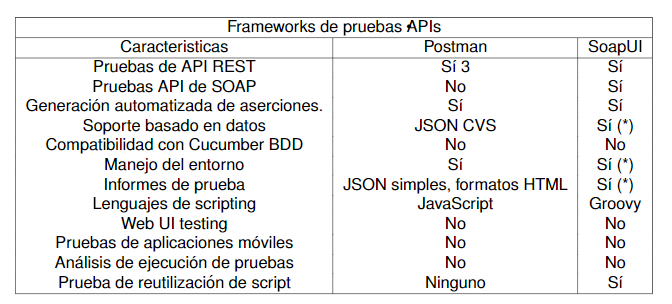
\includegraphics[width=1\linewidth]{img/tabla.png}


  • (*) Solo se admite en la edición comercial.
\\ • REST y SOAPson los tipos de API dominantes, que representan mas del 95\% de 
todos los servicios web  API de acuerdo con el Informe de Estado de Integracion API. 
\\• Generacion automatizada de aserciones :esta capacidad implica analizar API y generar
 aserciones automaticamente. Se espera que ahorre tiempo al generar aserciones manualmente 
 para las API.
 \\ • Informes de prueba: las dos herramientas proporcionan capacidades para reportar resultados 
 de prueba de API. Postman genera informes en formatos JSON y HTML; Para SoapUI, la capacidad 
 de producir informes de prueba detallados se encuentra en la edicion comercial.
 \\•  Pruebas de UI web y aplicaciones moviles: en el desarrollo de una aplicacion multiplataforma, el equipo realiza pruebas de aplicaciones moviles y UI web ademas de las API de pruebas. 
\\•  Analisis de ejecucion : prueba los registros de exaccion de prueba.
\\• Lenguajes de scripting: todas las herramientas usan lenguaje basado en java.
\newpage

    


\section{Bibliografía}

\begin{thebibliography}{X}
  
  
  \bibitem{Baz} \textsc{Shane Hastie, S. H., \& Stéphane Wojewoda, S. W.} ,
  \textit{}(2015),Standish Group 2015 Chaos Report \- Q\&A with Jennifer Lynch. InfoQ.\url{https://www.infoq.com/articles/}
  
  \bibitem{Baz} \textsc{Valencia Altamirano, D. G. } ,
  \textit{}(2018),Análisis de frameworks de desarrollo de api rest y su impacto en el rendimiento de aplicaciones web con arquitectura Spa (Master's thesis).\url{http://repositorio.utn.edu.ec/handle/123456789/8264}

  \bibitem{Baz} \textsc{Microsoft. (s. f.). Códigos de error de la API REST} ,
  \textit{}MicrosoftDocs. Recuperado 2 de diciembre de 2020, de:\url{https://docs.microsoft.com/es-es/partner/develop/}

  \bibitem{Baz} \textsc{¿Qué es la automatización de pruebas de API?} ,
  \textit{}(2020), Guru99.  \url{https://www.guru99.com/api-testing.html}

  \bibitem{Baz} \textsc{López, A.} ,
  \textit{}(2020),Qué es Postman y para qué sirve. OpenWebinars.net. de: \url{https://openwebinars.net/blog/que-es-postman/}

  \bibitem{Baz} \textsc{Federico Toledo } ,
  \textit{}(2020),API testing con Postman y SoapUI. de: \url{https://www.federico-toledo.com/api-testing-con-postman-y-soapui/}

  \bibitem{Baz} \textsc{Kumarasinghe, C. U., Liyanage, K. L. D. U., Madushanka, W. A. T., \& Mendis, R. A. C. L. } ,
  \textit{}(2016),Performance Comparison of NoSQL Databases in Pseudo Distributed Mode: Cassandra, MongoDB \& Redis.

\newpage
  \bibitem{Baz} \textsc{SoapUi | Marco de Desarrollo de la Junta de Andalucía. } ,
  \textit{}\url{ttp://www.juntadeandalucia.es/}. Recuperado 4 de diciembre de 2020, de \url{http://www.juntadeandalucia.es/servicios/madeja/contenido/recurso/209}

\end{thebibliography}


\end{document}